% Relatório — Trabalho Prático de Laboratórios de Informática 2025/26
% Compilar com:  pdflatex main -> bibtex main -> pdflatex main -> pdflatex main
%           ou:  latexmk -pdf main.tex
\documentclass[11pt,a4paper]{report}

\usepackage[portuguese]{babel}
\usepackage[utf8]{inputenc}
\usepackage[T1]{fontenc}
\usepackage{graphicx}
\usepackage{hyperref}
\usepackage{listings}
\usepackage{xcolor}
\usepackage{tikz}          % para o grafo da hierarquia de pastas
\usepackage{caption}

% estilo básico para listagens de código
\lstset{
  basicstyle=\ttfamily\small,
  keywordstyle=\color{blue},
  commentstyle=\color{gray},
  frame=single,
  breaklines=true,
  showstringspaces=false,
}

\title{Trabalho Prático\\\large Análise de Débitos Diretos (PS2)}
\author{Grupo 99 \\ A1 --- ... \\ A2 --- ... \\ A3 --- ...}
\date{Laboratórios de Informática --- LESI/LESIPL --- 2025/26}

\begin{document}

\maketitle

% ------------ índices (obrigatórios no enunciado) ------------
\tableofcontents
\listoffigures
\listoftables
\lstlistoflistings

% ------------------------ capítulos --------------------------
\chapter{Introdução}
% Contexto, objetivos do trabalho e organização do documento.
% Usar \emph{ênfase}, \textbf{negrito} e \textit{itálico} ao longo do texto.

\chapter{Formato PS2 e Leitura dos Dados}
% Descrever o formato simplificado e a estratégia de leitura.
% Incluir aqui uma listagem de código, ex.:
%
% \begin{lstlisting}[language=Python,caption={Listagem de ficheiros},label=lst:listar]
% def listar_ficheiros_ps2(pasta):
%     return sorted(Path(pasta).glob("DD_*.ps2"))
% \end{lstlisting}
%
% referida no texto como Listagem~\ref{lst:listar}.

\chapter{Validação}
% Validação de estrutura, NIF (Anexo A) e NIB (Anexo B).
% Incluir uma tabela, ex.:
%
% \begin{table}[h]\centering
%   \begin{tabular}{lcc}
%     Ficheiro & Estrutura & NIF/NIB \\ \hline
%     ...      & OK        & ...     \\
%   \end{tabular}
%   \caption{Resultados da validação}\label{tab:validacao}
% \end{table}

\chapter{Dashboard}
% Descrição da solução Shiny e das vistas implementadas.
% Incluir uma figura (captura de ecrã), ex.:
%
% \begin{figure}[h]\centering
%   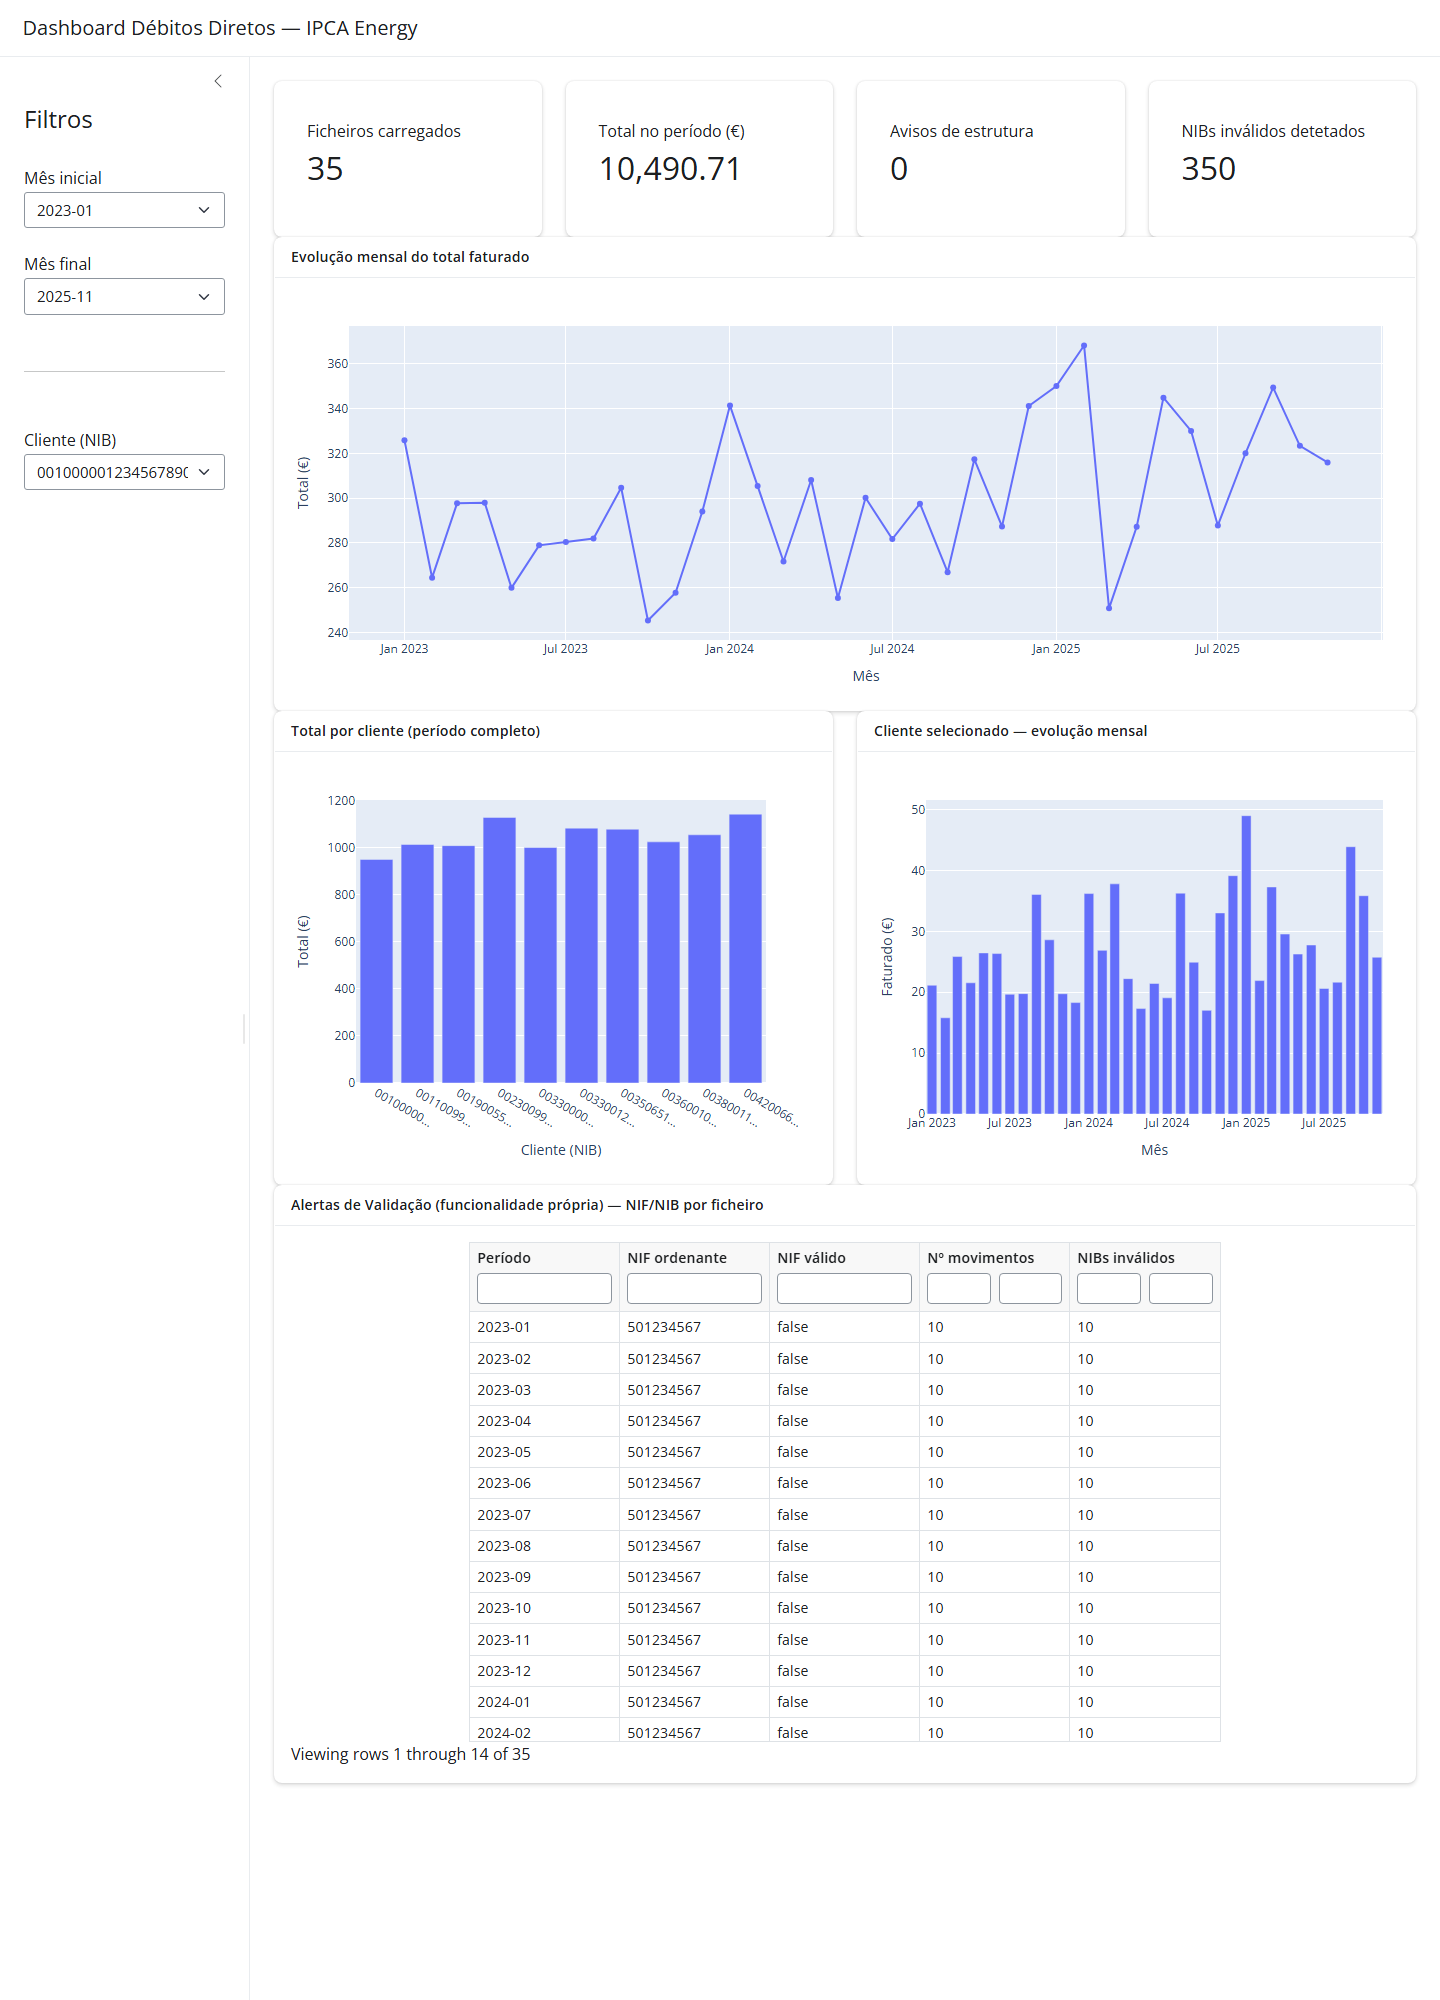
\includegraphics[width=0.8\textwidth]{img/dashboard.png}
%   \caption{Vista principal do dashboard}\label{fig:dashboard}
% \end{figure}

\chapter{Organização do Projeto}
% Aqui inclui-se o grafo TikZ da hierarquia de pastas (pedido no enunciado).
\begin{figure}[h]\centering
\begin{tikzpicture}[every node/.style={draw,rounded corners,font=\small},
                    level distance=10mm, sibling distance=22mm]
  \node {projeto-ps2}
    child { node {data} }
    child { node {src}
      child { node {ps2} }
    }
    child { node {docs} };
\end{tikzpicture}
\caption{Hierarquia de pastas do projeto}\label{fig:arvore}
\end{figure}

\chapter{Conclusão}
% Síntese, dificuldades e trabalho futuro.

% ------------------------ bibliografia -----------------------
\bibliographystyle{plain}
\bibliography{referencias}

\end{document}
